\section{Disaggregated Computing Architecture}
\label{ch:background:disaggregated}



\begin{figure}[t]
  \centering
    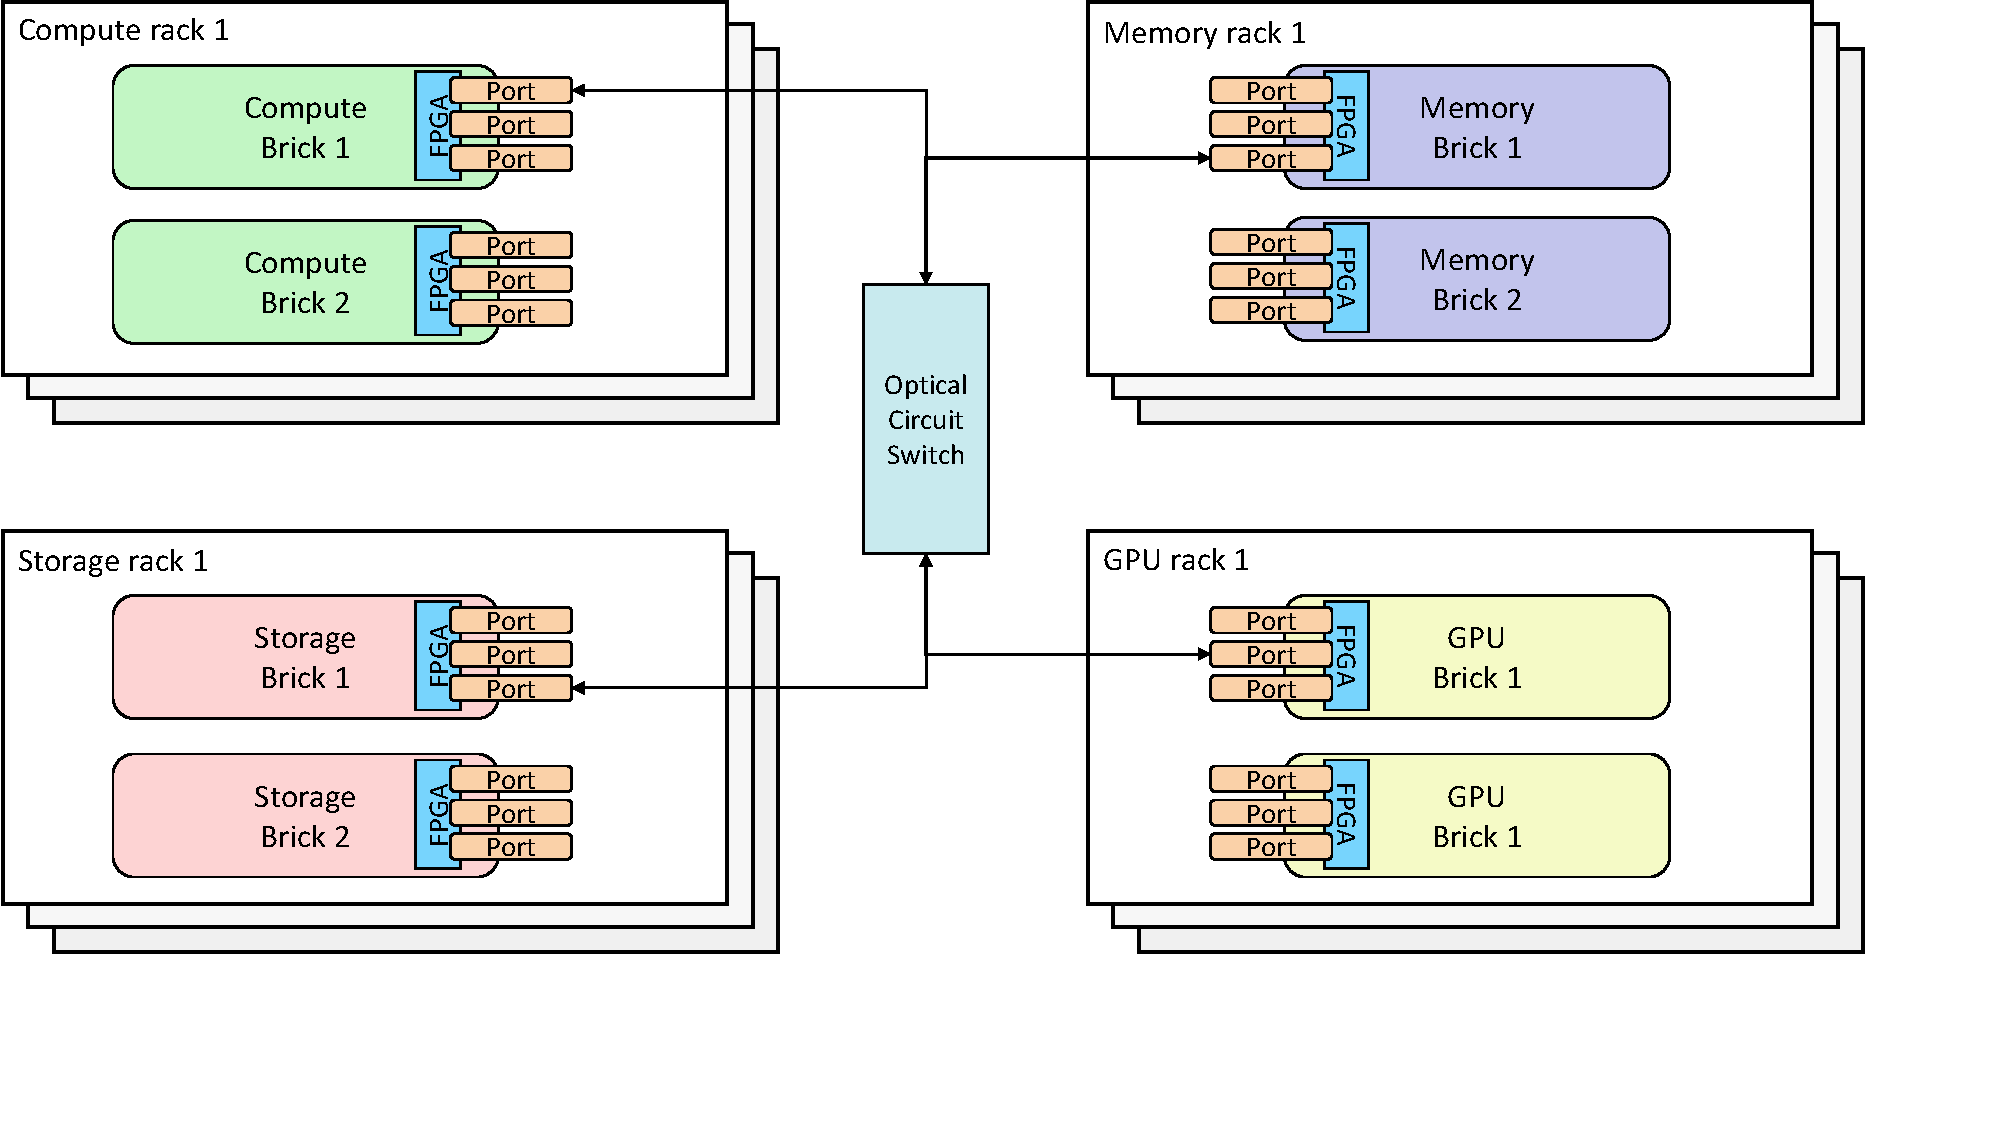
\includegraphics[trim={0 2cm 2cm 0},clip,width=\linewidth]{chapters/background/figures/disaggregated.pdf}
    \caption[Disaggregated architecture similar to dReDBox project]{\textbf{Disaggregated architecture similar to dReDBox project~\cite{dis1}.} The figure shows an example disaggregated architecture similar to dReDBox project~\cite{dis1} that are common in modern data centers. Rather than fully-fledged computers, the architecture employs different racks - compute, memory, storage etc. Inside this racks, there are multiple special purpose SoC-based microservers that are called bricks. These bricks have communication ports to talk to other bricks over fast optical circuit switches.}
    \label{fig:disagg_bg}
\end{figure}


Traditional computing hardware is built around the concept of motherboard-as-a-unit (or mainboard), where a motherboard has one or multiple CPU sockets, DRAM slots, PCI express ports to plug expansion cards for storage, accelerators, networks, etc. Many of the legacy data centers employs such integrated server racks  (e.g., Dell PowerEdge rack server~\cite{rack_server_dell}, Lenovo Blade server~\cite{rack_server_lenovo}, etc.). However, such systems are not fully flexible, e.g., one needs to allocate a new server rack to expand the DRAM if existing racks are already at their maximum capacity. Such a way to resource allocation/revocation is further complicated because not all VM instances are equal. Some of them are CPU-intensive, while others could be storage or memory or GPU intensive. In order to have a flexible allocation of resources all-around a data center, many of the modern data centers are moving to the disaggregated architecture where the resources (CPU, memory, storage, GPUs, etc.) are \emph{disaggregated}. One such example architecture is dReDBox project~\cite{dis1,dis2} that is also shown in Figure~\ref{fig:disagg_bg}. Such an architecture is flexible and demand-driven. For example, if a VM requires more memory, Memory bricks can be allocated to the VM dynamically~c\cite{lim2009disaggregated}. After the computation, these bricks can be revoked and utilized in other workloads. Similar could be done for other resources such as GPUs, accelerators, etc. All of these specialized racks are connected over a very low-latency optical network and provides an abstraction of all the data center resources. A summary of different disaggregated computing proposal can be found in~\cite{meyer2017disaggregated}.

On the commercial space, disaggregated computing model is well-adopted. Some of the notable examples are Amazon Elastic Cloud (EC2)~\cite{ec2}, Microsoft Azure high performance computing (HPC) cloud~\cite{azure}, NetApp HCI~\cite{netapp} and many more. DPU or data processing units~\cite{dpu} are the key component of such flexible, high-scalable disaggregated architecture. DPUs are SoC based programmable processors that typically\footnote{DPUs from different manufacturers differ widely. The following description is how Nvidia defines DPU.} contains the following:

\begin{itemize}
  \item ARM-based multi-core processor.
  \item High-performance network interfaces. 
  \item A rich set of flexible and programmable acceleration engines that are capable of executing complex ML or AI workloads.
\end{itemize}

These DPUs can be integrated into storage, network, or processing (CPU or GPU) nodes to make them self-sufficient. These nodes can talk to each other and combine themselves based on the workloads. Some of the well-deployed DPUs includes Nvidia BlueField 2~\cite{bluefield}, Fungible DPU platforms~\cite{fungible}, etc.